\documentclass{article}   	                         % use "amsart" instead of "article" for AMSLaTeX format
\usepackage{fullpage}                		% ... or a4paper or a5paper or ... 
\usepackage{enumerate}				% Use enumerate to list subsections
\usepackage{graphicx}				% Use pdf, png, jpg, or eps§ with pdflatex; use eps in DVI mode
\usepackage{fancyvrb}
\usepackage{algorithm}
\usepackage{algpseudocode}
\usepackage{amsmath}
\usepackage{dsfont}

\newcommand{\ra}{\rightarrow}

%SetFonts

\title{Computer System Fundamentals HW \#6}
\author{Quan Zhou}
\date{Mar 21st, 2016}
\begin{document}
\maketitle
\section*{Problem 1}
\begin{enumerate}[(a)]
\item
Since the Highest Slowdown Next (HSN) scheduler tries to select the job with the maximum slowdown, therefore preventing longer jobs from keeping waiting, jobs with short CPU burst times will be postponed. For a system where I/O bound jobs are requested frequently, HSN scheduler would be unfair to these short jobs as the scheduler ranks jobs by slowdown, which is the ratio of $\frac{T_q}{T_s}$. 
\item
Preemption at job arrival times would not be a good solution because the current job whether a long or short job will be interrupted by the highest slowdown job in the queue. As the scheduler would give priority to the newly arrived and the highest slowdown job, short jobs (I/O bound jobs) won't be executed efficiently: any short job that is currently running will be interrupted by higher-slowdown jobs, resulting in a long time to be executed.
\item
With a fixed timeout, it would be fairer to both long and short jobs: in the above example: short job would be forced to execute should it exceed preemption timeout. This allows the scheduler to control response times by preventing certain long jobs running for too long in order to let another process run.Though depending on the settings for the "timeout",  in situations when short jobs are arriving frequently, they would still pay the cost (of waiting) for longer jobs.
\item
To improve the preemptive scheduler based of HSN,
\end{enumerate}
\section*{Problem 2}
\begin{enumerate}[(a)]
\item
By examining the above code, one fatal problem is the critical sections is accessible to both $P_0$ and $P_1$ whenever it is their turn: the critical section is accessed after the loop where the flag is set up and the turn is checked. Notice the end of the loop basically only sets $\text{flag[i] :=true }$. I tried to run $P_0$ first and then $P_1$ arrives right before the line $\text{if flag[1]\{}$. We have line by line code until the following and realize both $P_0$ and $P_1$ can access the critical section.\\
\begin{center}
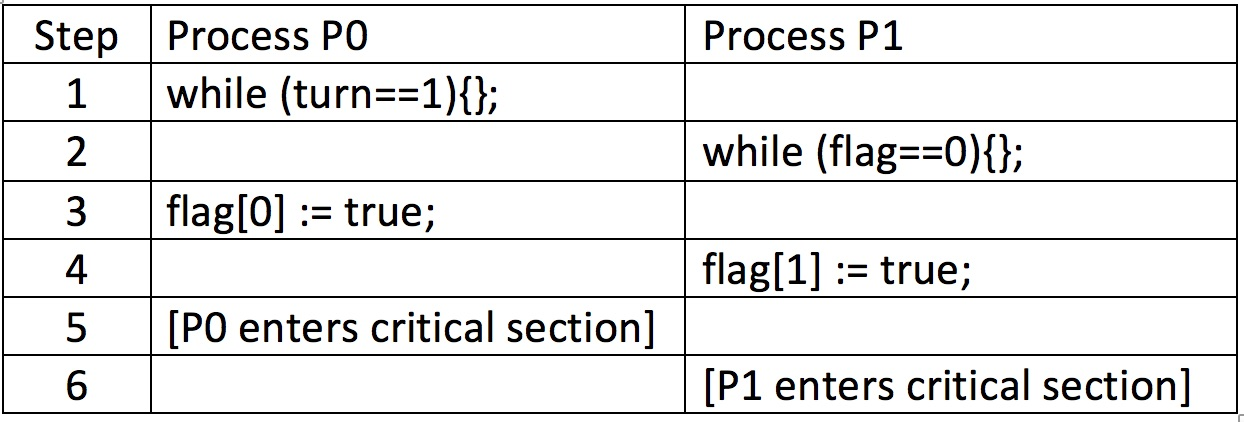
\includegraphics[scale = 0.2]{Picture1.jpg}
\end{center}
\item
The following code should fix the bug and mutual exclusion is achieved (based of Dekker's Algorithm):
\begin{algorithm}
\caption{Dekker's Algorithm}\label{Process P0}
\begin{algorithmic}
   \State Process P0:
   \Repeat
    \State flag[0]:=true;
    \While {flag[1]}
     \If {turn==1}
      \State flag[0]:=false;
      \While {turn==1}
       \State waiting
      \EndWhile
      \State flag[0]:=true;
    \EndIf
    \EndWhile
    \State{Critical section}
    \State turn[1]:=true;
    \State flag[0]:=false;
      \State       \text {Remainder section}
   \Until {forever}
\end{algorithmic}
\end{algorithm}
And like wise for Process P1, we have:\\
\begin{algorithm}
\caption{Dekker's Algorithm}\label{Process P1}
\begin{algorithmic}
   \State Process P1:
   \Repeat
    \State flag[1]:=true;
    \While {flag[0]}
     \If {turn==0}
      \State flag[1]:=false;
      \While {turn==0}
       \State waiting
      \EndWhile
      \State flag[1]:=true;
    \EndIf
    \EndWhile
    \State{Critical section}
    \State turn[0]:=true;
    \State flag[1]:=false;
      \State       \text {Remainder section}
   \Until {forever}
\end{algorithmic}
\end{algorithm}
\end{enumerate}
\section*{Problem 3}
\begin{enumerate}[(a)]
\item Codes see src folder and output for each part is in log folder.\\
\item Codes see src folder and output for each part is in log folder.\\
\item Yes. I did two different runs:\\
1. k < 6 and sleep for 20 msec for each printed message\\
The output shows the threads being served in the following order:
0 0 1 0 1 0 0 1 1 1.\\
During thread 0's entries, thread 1 was able to access through the critical section twice.\\
2. k < 30 and sleep for 20-40 msec for each printed message\\
The output shows the threads being served in the following order:\\
0 0 1 0 1 0 0 0 0 0 0 0 0 0 0 0 0 0 0 0 0 0 0 0 0 0 0 0 0 0 0 1 1 1 1 1 1 1 1 1 1 1 1 1 1 1 1 1 1 1 1 1 1 1 1 1 1 1\\
Again during thread 0's entries, thread 1 was able to access through the critical section twice.\\
\item
Codes see src folder and output for each part is in log folder. we see that the scenario in (c) does not occur in Peterson's Algorithm.\\
\end{enumerate}
\section*{Problem 4}
\begin{BVerbatim}
See src folder for codes
\end{BVerbatim}
\\
I did 100 samples/runs of the code where thread 0 and 1 execute the while loop defined by Peterson's algorithm. I took the average and computed the $s$ (sample standard deviation) and hence the 95$\%$ confidence interval for each thread:\\
\begin{center}
The estimated times the "while" loop is accessed during the multi-thread processing:\\
Thread 0: (115.79, 113.57)\\
Thread 1: (111.55, 133.03)\\

\begin{BVerbatim}
in millions times
\end{BVerbatim} 
\end{center}

\end{document}